\documentclass[../thesis.tex]{subfiles}

\begin{document}

\chapter{Vertex reconstruction details}
\label{chap:vertexReconDetails}

The AdSimple vertex reconstruction proceeds in multiple stages \cite{adsimple1,adsimple2}, as shown in \autoref{fig:vtx_rec_flow}. First, an initial vertex is determined by taking a simple \emph{center of charge} (COC) using the coordinates of the PMTs. As this method suffers from significant biases (largely toward the center of the AD), a correction is then applied, based on interpolating a map of the mean bias (as a function of COC position) determined from a sample of Monte Carlo events, giving the \emph{Monte Carlo Corrected COC} (MCC-COC). However, even with the MC correction, this vertex still suffers from biases, particularly at large $z$ (\autoref{fig:reconMccCocWiggles}). In order to reduce such effects, and to also improve the resolution of the position reconstruction, a final vertex is computed by matching the distribution of PMT charges to a library of MC templates. We now discuss these steps in further detail. 

\begin{figure}[h]
  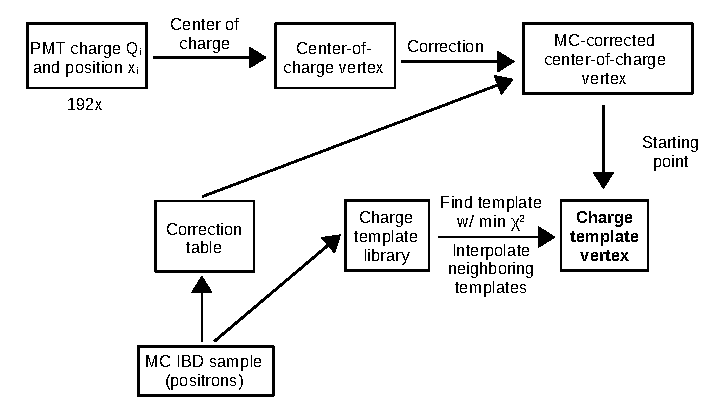
\includegraphics[scale=1.0]{Reconstruction/vtx_rec_flow.pdf}
  \caption{Flowchart of the steps involved in the AdSimple vertex reconstruction.}
  \label{fig:vtx_rec_flow}
\end{figure}


\begin{figure}[h]
  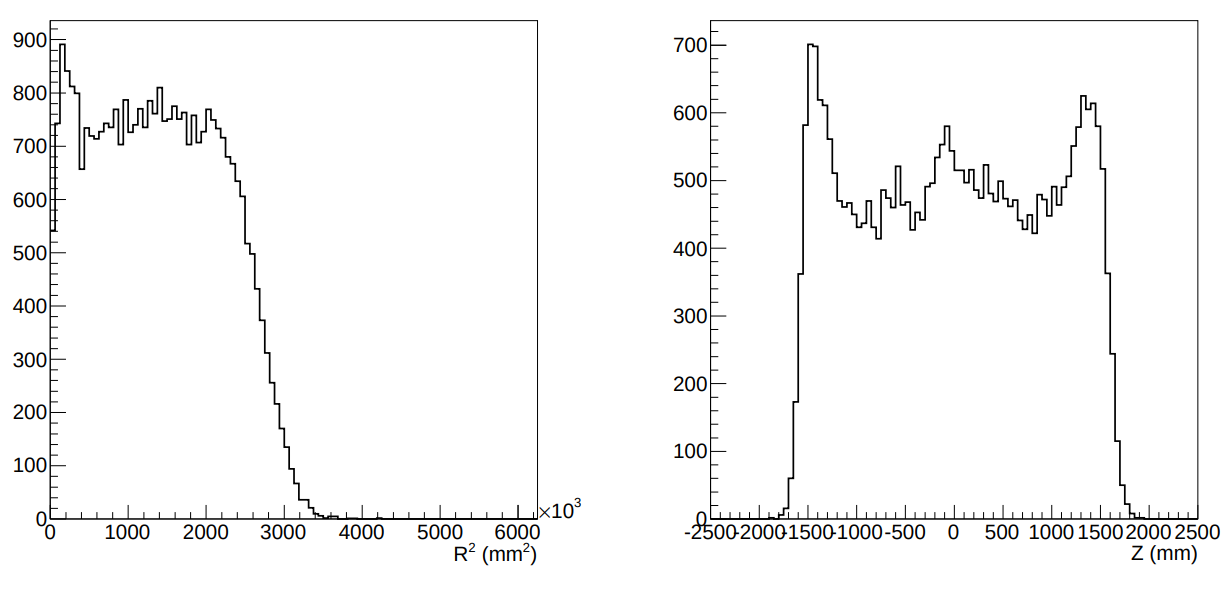
\includegraphics[scale=0.4]{Reconstruction/mcc_coc_wiggles_positron.png}
  \caption{Biases in the MCC-COC vertex distributions for positrons associated with IBD neutrons. The true distribution of events is uniform in the GdLS. From \cite{adsimple1}.}
  \label{fig:reconMccCocWiggles}
\end{figure}

The COC vertex is calculated trivially,
\begin{equation}
  x_{\mathrm{COC}} = \frac{\sum_{i}^{\mathrm{PMTs}} Q_i \vec{x_i}}{\sum_i^{\mathrm{PMTs}} Q_i},
\end{equation}
where $\vec{x_i}$ is the position of the $i$th PMT (in Cartesian coordinates, with the origin at the AD's center), and $Q_i$ is the corresponding observed charge in photoelectrons (without any correction for electronics nonlinearity). To this vertex, the correction from MC is applied next.

The MC sample consists of a large number of uniformly-distributed IBD events, generated using the ILL-Vogel flux model without oscillation (see \autoref{tab:mccCocMcSampleCoefs}). A cut is applied on the true interaction to eliminate events that occur outside the OAV. The positrons (i.e. prompt triggers) from these events are then used to generate a correction table.

\begin{table}[h]
  \begin{tabular}{lr}
    \toprule
    Isotope & Fraction \\
    \midrule
    $^{235}$U & 0.60 \\
    $^{238}$U & 0.05 \\
    $^{239}$Pu & 0.30 \\
    $^{241}$Pu & 0.05 \\
    \bottomrule
  \end{tabular}
  \caption{Nominal fission fractions used when employing the ILL-Vogel model to generate simulated IBD events for constructing the MC correction table for the MCC-COC.}
  \label{tab:mccCocMcSampleCoefs}
\end{table}

For each MC event, the COC vertex is calculated, and two corrections, a ``radial'' and a ``vertical'' one, are computed (using cylindrical coordinates, again with the origin at the AD's center):
\begin{equation}
  \Delta r = \frac{\vec{r}_{\mathrm{true}} \cdot \vec{r}_{\mathrm{COC}}}{\abs{\vec{r}_{\mathrm{COC}}} - r_{\mathrm{COC}}},
\end{equation}
\begin{equation}
  \Delta z = z_{\mathrm{true}} - z_{\mathrm{COC}},
\end{equation}
Events are divided into 20 bins for $\SI{0}{m} < r_{\mathrm{COC}} < \SI{2}{m}$ and 40 bins for $\SI{-2}{m} < z_{\mathrm{COC}} < \SI{2}{m}$. For each bin, the mean $\Delta z$ is computed, while the mean $\Delta r$ is computed over (and assigned to) all $z{_\mathrm{COC}}$ bins for a given $r_{\mathrm{COC}}$, since there is very little $z$ dependence on $\Delta r$. The $\Delta r$ and $\Delta z$ correction tables are ``pre-interpolated'' with a spline function\footnote{Unfortunately, it was not possible to find a record of the exact spline function used. Presumably, it was a quadratic or cubic function. In any case, since the MCC-COC is ultimately only used as a ``pre-fit'' starting point for the template-based reconstruction, its precise details are not extremely important.} to give a $\times$10-finer grid, which is then stored for use by AdSimple. During reconstruction, linear interpolation is applied to this fine-binned grid to look up the corrections for arbitary ($r_{\mathrm{COC}}$, $z_{\mathrm{COC}}$). Application of the correction is trivial: $r \mapsto r + \Delta r$ and $z \mapsto z + \Delta z$. This gives the MCC-COC vertex.

The final stage of the AdSimple vertex reconstruction relies on a library of 9,600 charge templates (i.e. distributions of charge across the PMTs), with each template corresponding to a voxel of the detector. These voxels (i.e. bins) are defined as the product of 20 bins in $\SI{0}{\square m} < r^2 < 2^2\;\mathrm{m}^2$, 20 bins in $\SI{-2}{m} < z < \SI{2}{m}$, and 24 bins in $0 < \phi < 2\pi$. The charge template for each voxel is taken from the mean of the charge distributions (each normalized by total charge) of all MC events whose true position lay within the voxel. The MC sample, in turn, is of the same nature as the one used for the COC correction: IBD positrons lying within the OAV. Taking advantage of the azimuthal symmetry of the detector response, each event was rotated in angular steps of $\pi/12$ to produce 23 ``clones'', which were added to the sample, thereby providing a ``free'' boost in statistics without the need to generate additional MC events.\footnote{In principle, the detector response is not completely azimuthally symmetric, due to the Earth's magnetic field. However, such effects are largely canceled by the conical magnetic shields around each PMT. Furthermore, the MC does not take this factor into account; thus, azimuthal symmetry is a valid assumption for the MC sample.}

\newcommand\Niobs{N_i^{\mathrm{obs}}}
\newcommand\Niexp{N_i^{\mathrm{exp}}}

During reconstruction, the charge templates are compared to the event's (normalized) charge distribution (again without correcting for electronics NL) using the ``$\chi^2$'' (more precisely, the log-likelihood)
\begin{align*}
  \chi^2 &= \sum_i^{\mathrm{PMTs}}\left[ -2 \ln \frac{P(\Niobs, \Niexp(r^2, z, \phi))}
        {P(\Niobs, \Niobs)} \right] \\
      &= 2 \sum_i^{\mathrm{PMTs}} \left[ \Niexp - \Niobs+ \Niobs \ln \left( \frac{\Niobs}{\Niexp} \right) \right],
\end{align*}
where $P(n, \nu) = \nu^n e^{-n} / (n!)$ is the Poisson probability of observing $n$ events when $\nu$ are expected. The MCC-COC vertex is used as a starting point to search the grid for a local minimum (which is presumably also a global minimum). Having thus located the bin with the lowest $\chi^2$, the reconstruction proceeds by quadratically interpolating the $\chi^2$ values at the neighboring grid points. This interpolation is performed independently for the three coordinates $r^2$, $z$, and $\phi$, each time using two neighbors in the appropriate direction. Letting $s$ to denote any of the three coordinates, with $s_1$ being the value of $s$ at the $\chi^2$-minimizing grid point, and $s_2$ and $s_3$ being those of the neighbors, the value of $s$ at the interpolated minimum is
\begin{equation}
  s_{\mathrm{min}} = \frac{(s_1^2 - s_2^2)(\chi_3^2 - \chi_1^2) - (s_1^2 - s_3^2)(\chi_2^2 - \chi_1^2)}{2(s_1 - s_2)(\chi_3^2 - \chi_1^2) - 2(s_1 - s_3)(\chi_2^2 - \chi_1^2)}.
\end{equation}
Calculated in this manner, $r_{\mathrm{min}}$, $z_{\mathrm{min}}$, and $\phi_{\mathrm{min}}$ give the final AdSimple reconstructed vertex. This vertex provides a significantly improved resolution compared to the MCC-COC vertex, of $\sim$7~cm in $r$ (\autoref{fig:chargeTemp_bias_r}) and $\sim$9~cm in $z$ (\autoref{fig:chargeTemp_bias_z}), compared to 11.5~cm (\autoref{fig:mccCoc_bias_r}) and 17~cm (\autoref{fig:mccCoc_bias_z}), respectively, for the MCC-COC. (These values are for IBD positrons.) There are also no significant biases within the OAV region; although some high-frequency ``wiggles'' remain (as a consequence of the finite grid spacing), these are insignificant in the context of performing physics analysis, as shown, for instance, by the consistency of physics results between AdSimple and AdScaled (which lacks such structures).

\begin{figure}[h]
  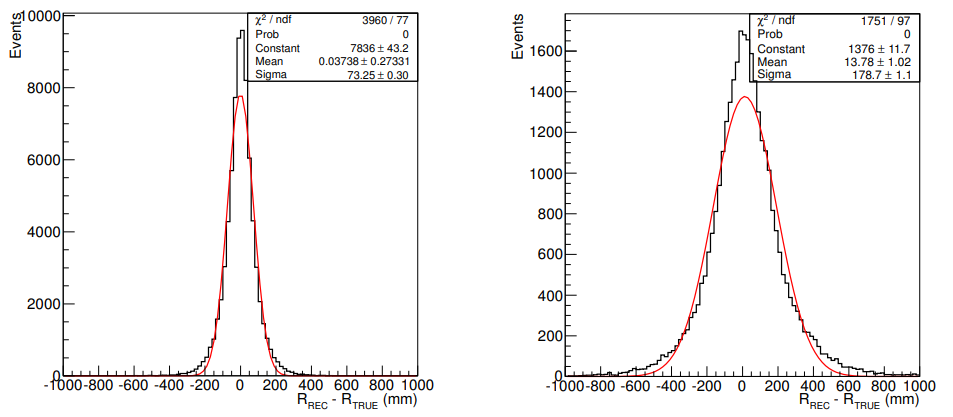
\includegraphics[scale=0.6]{Reconstruction/chargeTemp_bias_r.png}
  \caption{Distributions of residuals of the radial coordinate for the AdSimple charge template vertex reconstruction. IBD positrons are shown on the left, while IBD nGd captures are shown on the right.}
  \label{fig:chargeTemp_bias_r}
\end{figure}

\begin{figure}[h]
  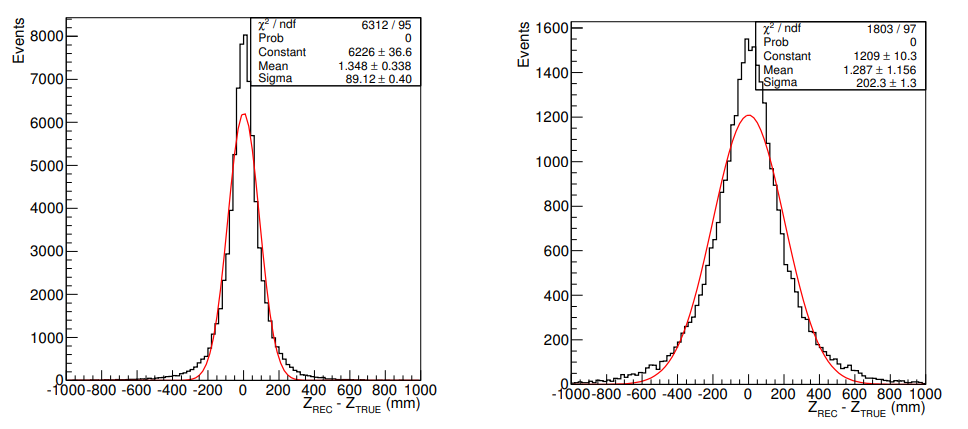
\includegraphics[scale=0.6]{Reconstruction/chargeTemp_bias_z.png}
  \caption{Distributions of residuals of the vertical coordinate for the AdSimple charge template vertex reconstruction. IBD positrons are shown on the left, while IBD nGd captures are shown on the right.}
  \label{fig:chargeTemp_bias_z}
\end{figure}

\begin{figure}[h]
  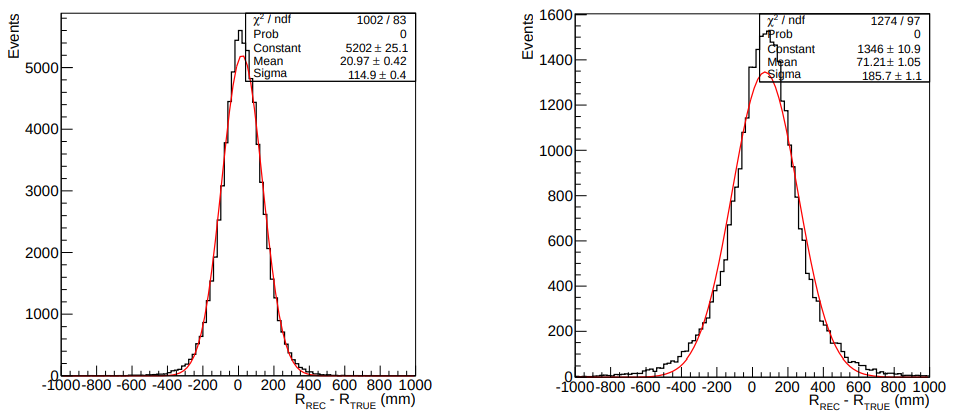
\includegraphics[scale=0.6]{Reconstruction/mccCoc_bias_r.png}
  \caption{Distributions of residuals of the radial coordinate for the AdSimple MC-corrected center of charge vertex. IBD positrons are shown on the left, while IBD nGd captures are shown on the right.}
  \label{fig:mccCoc_bias_r}
\end{figure}

\begin{figure}[h]
  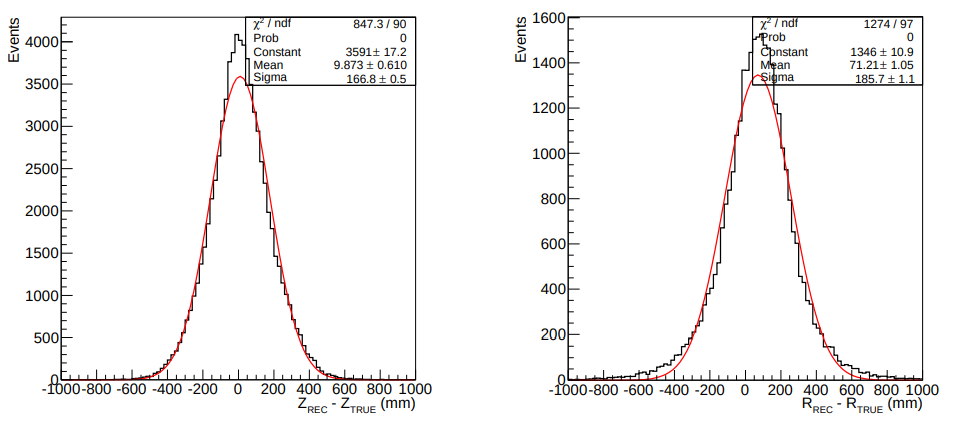
\includegraphics[scale=0.6]{Reconstruction/mccCoc_bias_z.png}
  \caption{Distributions of residuals of the vertical coordinate for the AdSimple MC-corrected center of charge vertex. IBD positrons are shown on the left, while IBD nGd captures are shown on the right.}
  \label{fig:mccCoc_bias_z}
\end{figure}

Note that the reconstructed vertex is not directly used in selecting IBD candidates in this analysis. However, it is still used indirectly in calculating the reconstructed energy (via the nonuniformity correction). In addition, some studies of background rates and spectra also depended on the reconstructed vertex. Finally, there is an independent oscillation analysis (not covered in this thesis), based on selecting IBDs where the neutron is captured on hydrogen, and this one typically relies on the use of the prompt-delayed distance in order to reduce the background of accidental coincidences.

\end{document}
